% Options for packages loaded elsewhere
\PassOptionsToPackage{unicode}{hyperref}
\PassOptionsToPackage{hyphens}{url}
\PassOptionsToPackage{dvipsnames,svgnames*,x11names*}{xcolor}
%
\documentclass[
  16pt,
]{krantz}
\usepackage{amsmath,amssymb}
\usepackage{lmodern}
\usepackage{ifxetex,ifluatex}
\ifnum 0\ifxetex 1\fi\ifluatex 1\fi=0 % if pdftex
  \usepackage[T1]{fontenc}
  \usepackage[utf8]{inputenc}
  \usepackage{textcomp} % provide euro and other symbols
\else % if luatex or xetex
  \usepackage{unicode-math}
  \defaultfontfeatures{Scale=MatchLowercase}
  \defaultfontfeatures[\rmfamily]{Ligatures=TeX,Scale=1}
  \setmonofont[Scale=0.7]{Source Code Pro}
\fi
% Use upquote if available, for straight quotes in verbatim environments
\IfFileExists{upquote.sty}{\usepackage{upquote}}{}
\IfFileExists{microtype.sty}{% use microtype if available
  \usepackage[]{microtype}
  \UseMicrotypeSet[protrusion]{basicmath} % disable protrusion for tt fonts
}{}
\makeatletter
\@ifundefined{KOMAClassName}{% if non-KOMA class
  \IfFileExists{parskip.sty}{%
    \usepackage{parskip}
  }{% else
    \setlength{\parindent}{0pt}
    \setlength{\parskip}{6pt plus 2pt minus 1pt}}
}{% if KOMA class
  \KOMAoptions{parskip=half}}
\makeatother
\usepackage{xcolor}
\IfFileExists{xurl.sty}{\usepackage{xurl}}{} % add URL line breaks if available
\IfFileExists{bookmark.sty}{\usepackage{bookmark}}{\usepackage{hyperref}}
\hypersetup{
  pdftitle={Matemáticas básicas},
  pdfauthor={Ricardo Michel MALLQUI BAÑOS},
  colorlinks=true,
  linkcolor=Maroon,
  filecolor=Maroon,
  citecolor=Blue,
  urlcolor=Blue,
  pdfcreator={LaTeX via pandoc}}
\urlstyle{same} % disable monospaced font for URLs
\usepackage{longtable,booktabs,array}
\usepackage{calc} % for calculating minipage widths
% Correct order of tables after \paragraph or \subparagraph
\usepackage{etoolbox}
\makeatletter
\patchcmd\longtable{\par}{\if@noskipsec\mbox{}\fi\par}{}{}
\makeatother
% Allow footnotes in longtable head/foot
\IfFileExists{footnotehyper.sty}{\usepackage{footnotehyper}}{\usepackage{footnote}}
\makesavenoteenv{longtable}
\setlength{\emergencystretch}{3em} % prevent overfull lines
\providecommand{\tightlist}{%
  \setlength{\itemsep}{0pt}\setlength{\parskip}{0pt}}
\setcounter{secnumdepth}{5}
\usepackage[spanish,es-lcroman]{babel}
\usepackage{mathtools}
\usepackage{graphicx}
\usepackage{amsmath}
\usepackage{makeidx}
\makeindex
%\usepackage{showframe}
%\usepackage[a4paper]{geometry}
%\geometry{verbose,tmargin=3cm,bmargin=3cm,lmargin=3.5cm,rmargin=3cm}
\setlength\parindent{15pt}
\usepackage[singlelinecheck=off]{caption}

\usepackage{times}
\renewcommand{\rmdefault}{ptm}
%\usepackage[lite,subscriptcorrection,nofontinfo,zswash]{mtpro2}

\usepackage{graphicx}

% Determine if the image is too wide for the page.
\makeatletter
\def\ScaleIfNeeded{%
  \ifdim\Gin@nat@width>\linewidth
    \linewidth
  \else
    \Gin@nat@width
  \fi
}
\makeatother

% Resize figures that are too wide for the page.
%\let\oldincludegraphics\includegraphics
%\renewcommand\includegraphics[2][]{%
%  \oldincludegraphics[scale=0.85]{#2}
%}

\usepackage{amsthm}
\makeatletter
\def\thm@space@setup{%
  \thm@preskip=8pt plus 2pt minus 4pt
  \thm@postskip=\thm@preskip
}
\makeatother

\flushbottom

\frontmatter
\ifluatex
  \usepackage{selnolig}  % disable illegal ligatures
\fi
\usepackage[]{natbib}
\bibliographystyle{apalike}

\title{Matemáticas básicas}
\author{Ricardo Michel MALLQUI BAÑOS}
\date{2022-06-13}

\usepackage{amsthm}
\newtheorem{theorem}{Teorema}[chapter]
\newtheorem{lemma}{Lema}[chapter]
\newtheorem{corollary}{Corolario}[chapter]
\newtheorem{proposition}{Proposición}[chapter]
\newtheorem{conjecture}{Conjectura}[chapter]
\theoremstyle{definition}
\newtheorem{definition}{Definición}[chapter]
\theoremstyle{definition}
\newtheorem{example}{Ejemplo}[chapter]
\theoremstyle{definition}
\newtheorem{exercise}{Ejercicio}[chapter]
\theoremstyle{definition}
\newtheorem{hypothesis}{Hypothesis}[chapter]
\theoremstyle{remark}
\newtheorem*{remark}{Observación}
\newtheorem*{solution}{Solución}
\begin{document}
\maketitle

%\cleardoublepage\newpage\thispagestyle{empty}\null
%\cleardoublepage\newpage\thispagestyle{empty}\null
%\cleardoublepage\newpage
\thispagestyle{empty}
\begin{flushright}
Universidad Nacional San Cristobal de Huamanga

Fisart.cf

Agradecimento a los estudiantes de la ESFAPA FGPA

A la UNSCH


\includegraphics[height=3cm]{U.pdf}
\end{flushright}
%\setlength{\abovedisplayskip}{-5pt}
%\setlength{\abovedisplayshortskip}{-5pt}

{
\hypersetup{linkcolor=}
\setcounter{tocdepth}{2}
\tableofcontents
}
\listoftables
\listoffigures
\newcommand{\N}{\mathbb{N}}
\newcommand{\R}{\mathbb{R}}
\newcommand{\CC}{\mathbb{C}}
\newcommand{\I}{\mathbb{I}}
\newcommand{\f}{\mathbb{f}}
\newcommand{\X}{\mathbb{X}}
\newcommand{\D}{\mathbb{D}}
\newcommand{\Z}{\mathbb{Z}}
\newcommand{\Q}{\mathbb{Q}}
\newcommand{\norm}[1]{\left\Vert#1\right\Vert}
\newcommand{\abs}[1]{\left\vert#1\right\vert}
\newcommand{\set}[1]{\left\{#1\right\}}
\newcommand{\seq}[1]{\left<#1\right>}
\newcommand{\co}[1]{\left[#1\right]}
\newcommand{\cc}[1]{\left(#1\right)}
\newcommand{\J}{\mathcal{J}}
\newcommand{\K}{\mathcal{K}}
\newcommand{\M}{\mathcal{M}}
\newcommand{\F}{\mathcal{F}}

\hypertarget{resumen}{%
\chapter*{Resumen}\label{resumen}}


La asignatura de Matemáticas Básicas forma parte del grupo de asignaturas básicas de primer curso, en todas las instituciones la cual tiene como objetivo principal desarrollar la capacidad de la resolución de problemas matemáticos sencillos que pueden plantearse en la escuela. Este carácter básico de la asignatura le confiere un papel clave en la formación de futuros egresados.

Este libro se divie en 9 capitulos: Logica, conjuntos, funciones y relaciones, numeros reales, funciones exponenciales y logaritmicas, induccion matematica, susceciones, numeros complejos, polinomios. Los cuales se desarrollarán conjuntas a ejemplos y ejercicios.

\hypertarget{introducciuxf3n}{%
\chapter*{Introducción}\label{introducciuxf3n}}


La matemática es una ciencia lógica deductiva, que utiliza símbolos para generar una teoría exacta de deducción e inferencia basada en definiciones, axiomas, postulados y reglas que transforman elementos primitivos en relaciones y teoremas más complejos. Esta ciencia enseña al individuo a pensar de una manera lógica y por lo tanto a desarrollar habilidades a resolver problemas y tomar decisiones. Las habilidades numéricas son valoradas por la mayoría de los sectores, se puede decir que en algunos casos son considerados esenciales.

La asignatura de Matemáticas Básicas forma parte del grupo de asignaturas básicas de primer curso, en todas las instituciones la cual tiene como objetivo principal desarrollar la capacidad de la resolución de problemas matemáticos sencillos que pueden plantearse en la escuela. Este carácter básico de la asignatura le confiere un papel clave en la formación de futuros egresados.

Capacidad para la resolución de los problemas matemáticos que puedan plantearse en la ingeniería. Aptitud para aplicar los conocimientos sobre: álgebra lineal; geometría; geometría diferencial; cálculo diferencial e integral; ecuaciones diferenciales y en derivadas parciales; métodos numéricos; algorítmica numérica; estadística y optimización.

Que los estudiantes hayan demostrado poseer y comprender conocimientos en un área de estudio que parte de la base de la educación secundaria general, y se suele encontrar a un nivel que, si bien se apoya en libros de texto avanzados, incluye también algunos aspectos que implican conocimientos procedentes de la vanguardia de su campo de estudio.

Capacidad para utilizar herramientas informáticas de búsqueda de recursos bibliográficos o de información relacionada con las telecomunicaciones y la electrónica. Resultados de aprendizaje (Objetivos formativos):

\begin{itemize}
\tightlist
\item
  Conocimiento de materias básicas y tecnologías, que le capacite para el aprendizaje de nuevos métodos y tecnologías, así como que le dote de una gran versatilidad para adaptarse a nuevas situaciones.
\item
  Capacidad de resolver problemas con iniciativa, toma de decisiones, creatividad, y de comunicar y transmitir conocimientos, habilidades y destrezas, comprendiendo la responsabilidad ética y profesional de la actividad del Ingeniero/a Técnico de Telecomunicación.
\end{itemize}

\mainmatter

\hypertarget{logica}{%
\chapter{Logica}\label{logica}}

\begin{theorem}[Pythagorean theorem]
\protect\hypertarget{thm:pyth}{}\label{thm:pyth}For a right triangle, if \(c\) denotes the length of the hypotenuse
and \(a\) and \(b\) denote the lengths of the other two sides, we have

\[a^2 + b^2 = c^2\]
\end{theorem}

\ref{thm:pyth}

\hypertarget{conjunciuxf3n}{%
\section{Conjunción}\label{conjunciuxf3n}}

\begin{longtable}[]{@{}
  >{\raggedright\arraybackslash}p{(\columnwidth - 12\tabcolsep) * \real{0.14}}
  >{\raggedright\arraybackslash}p{(\columnwidth - 12\tabcolsep) * \real{0.14}}
  >{\raggedleft\arraybackslash}p{(\columnwidth - 12\tabcolsep) * \real{0.14}}
  >{\raggedleft\arraybackslash}p{(\columnwidth - 12\tabcolsep) * \real{0.14}}
  >{\raggedleft\arraybackslash}p{(\columnwidth - 12\tabcolsep) * \real{0.14}}
  >{\raggedleft\arraybackslash}p{(\columnwidth - 12\tabcolsep) * \real{0.14}}
  >{\raggedleft\arraybackslash}p{(\columnwidth - 12\tabcolsep) * \real{0.14}}@{}}
\caption{\label{tab:ww} Conjunción.}\tabularnewline
\toprule
\(p\) & \(q\) & \(p\wedge q\) & \(p\vee q\) & \(p\Longrightarrow q\) & \(p\Longleftrightarrow q\) & \(p\Delta q\equiv \sim (p\Longleftrightarrow q)\) \\
\midrule
\endfirsthead
\toprule
\(p\) & \(q\) & \(p\wedge q\) & \(p\vee q\) & \(p\Longrightarrow q\) & \(p\Longleftrightarrow q\) & \(p\Delta q\equiv \sim (p\Longleftrightarrow q)\) \\
\midrule
\endhead
V & V & V & V & V & V & F \\
V & F & F & V & F & F & V \\
F & V & F & V & V & F & V \\
F & F & F & F & V & V & F \\
\bottomrule
\end{longtable}

\begin{figure}

{\centering 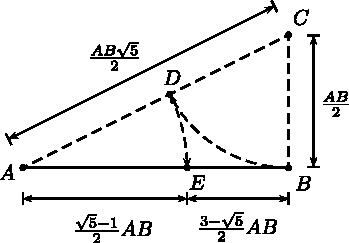
\includegraphics{aureo} 

}

\caption{wwwwwwwwww}\label{fig:ww1}
\end{figure}

\(\frac{\sqrt{5}-1}{2}AB\)
\[\frac{\sqrt{5}-1}{2}AB\]

Refiérase al cuadro \ref{tab:ww}

\hypertarget{conjuntos}{%
\chapter{Conjuntos}\label{conjuntos}}

\begin{definition}[Conjunto]
\protect\hypertarget{def:conjunto}{}\label{def:conjunto}Es una coleccion de elementos con características similares
\end{definition}

\hypertarget{determinaciuxf3n-de-un-conjunto}{%
\section{Determinación de un conjunto}\label{determinaciuxf3n-de-un-conjunto}}

\begin{definition}[Determinacion de conjuntos]
\protect\hypertarget{def:conjunto2}{}\label{def:conjunto2}Por extensión y comprensión.
\textbf{Extensión}
\[A=\left\{ 1,2,3,4,5,6,7 \right\} \]

\textbf{Comprensión}
\[A=\left\{ x \in \mathbb{N};0<x<5 \right\}  \]
\end{definition}

\hypertarget{conjuntos-buxe1sicos}{%
\section{Conjuntos básicos}\label{conjuntos-buxe1sicos}}

\begin{itemize}
\item
  Conjuntos universal
\item
  Conjunto de los sitemas numéricos
  \[
  \mathbb{N}, \mathbb{Z}, \mathbb{Q}, \mathbb{I}, \mathbb{R}, \mathbb{C}
  \]
\item
  Cojunto vacio
  \[
  \phi=\left\{x/x\neq x\right\}
  \]
\item
  Conjunto unitario
  \[
  A=\left\{a\right\}
  \]
\end{itemize}

\hypertarget{funciuxf3n-proposicional-y-cuantificadores}{%
\section{Función proposicional y cuantificadores}\label{funciuxf3n-proposicional-y-cuantificadores}}

\hypertarget{funciuxf3n-proposicional}{%
\subsection{Función proposicional}\label{funciuxf3n-proposicional}}

\begin{definition}[Función proposicional]
\protect\hypertarget{def:proposicional}{}\label{def:proposicional}Sea \(x\) una variable \(P(x)\) un \emph{enunciado}, \(P(x)\) es una \textbf{\emph{función proposicional}} si al sustituir la variable con una constante este se convierte en una \emph{proposición}.
\end{definition}

Por ejemplo \(P(x)\): \(x\) es un numero par

Al conjunto de todos lo valores de \(x\) se denomina \emph{domino de la variable}

\hypertarget{cuantificadores}{%
\subsection{Cuantificadores}\label{cuantificadores}}

\begin{definition}[Cuantificador existencial]
\protect\hypertarget{def:existencial}{}\label{def:existencial}Este cuatificador
\[\exists\]
Es una generalización de la disyunción Inclusiva. Por ello, es verdadero cuando al menos un valor de \(x\) perteneciente al Dominio de \(A\), es Verdadero. Se denota; \(\exists x / P (x)\) Se lee: ``Existe al menos un \(x\)'', ``Algunos \(x\)'', ``Hay \(x\)'', ``Existe un \(x\)'', etc.
\end{definition}

\begin{definition}[Cuantificador universal]
\protect\hypertarget{def:universal}{}\label{def:universal}Este cuatificador
\[\forall\]
Es una generalización de la \emph{conjunción}. Debido a esto es verdadero cuando todos los valores de \(x\) que pertenecen al Dominio de \(A\) son Verdaderos. Se denota: \(\forall x ; p(x)\) Se lee: ``Para Todo \(x\)'', ``Para cada \(x\)'', ``Todos (as) las \(x\)'', ``Todo \(x\)''.
\end{definition}

Sea \(A=\left\{1,2,3,4,5\right\}\) y la función proposicional \(3x-2<12\) entonces las proposiciones

\begin{enumerate}
\def\labelenumi{\arabic{enumi}.}
\tightlist
\item
  \(\forall x\in A:3x-1<14\)
\item
  \(\exists\; x\in A:3x-2<12\)
\end{enumerate}

son falsa y verdadera respectivamente

\begin{definition}[Proposición universal]
\protect\hypertarget{def:universal2}{}\label{def:universal2}Una \emph{proposición universal} es aquella que está provista de un \emph{cuantificador universal}, y tiene la forma: \[\forall x\in A:p(x)\]
\end{definition}

\begin{definition}[Proposición existencial]
\protect\hypertarget{def:existencial2}{}\label{def:existencial2}Una \emph{proposición existencial} es aquella que está provista de un \emph{cuantificador existencial}, y tiene la forma: \[\exists x\in A:p(x)\]
\end{definition}

Cambiando el cuantificador universal por el cuantificador existencial, o viceversa, es decir \[\sim[\exists x\in A; P(x)]\equiv\forall x\in A;\sim P(x)\]

\[
\sim\left[\forall  x\in A; P(x)\right]\equiv\exists\; x\in A;\sim P(x)
\]

La negación del \textbf{\emph{cuantificador universal}} es equivalente a la \emph{afirmación de un cuantificador existencial} respecto de la \textbf{\emph{función proposicional negada}.}

La negación de un \textbf{\emph{cuantificador existencial}} es equivalente a la \emph{afirmación de un cuantificador universal} respecto de la \textbf{\emph{función proposicional negada}}.

\begin{example}
\protect\hypertarget{exm:wwwwwwww}{}\label{exm:wwwwwwww}

Dada la proposición: ``Si todos los números primos son impa­res, los números positivos son mayores que -1''

\begin{itemize}
\tightlist
\item
  Expresarla simbólicamente
\item
  Negar oracionalmente la proposición
\end{itemize}

\end{example}

\begin{solution}

Sea \(p(x):\) números primos son impares y \(q(x):\) números positivos mayores que -1

\begin{itemize}
\item
  \(\forall x:[p(x)\rightarrow q(x)]\)
\item
  Negando el item anterior
  \[
  \begin{aligned}
  \sim\left\{\forall x:[p(x)\rightarrow q(x)]\right\}
  \equiv& \sim\left\{\forall x:p(x)\rightarrow \forall x:q(x)\right\}\\
  =&\sim\left\{\sim[\forall x:p(x)]\vee \forall x:q(x)\right\}\\
  \equiv&\quad\forall x:p(x)\wedge \exists\; x:\sim q(x)
  \end{aligned}
  \]
  que se lee: ``Todos los números primos son impares y algunos números no son mayores que -1''
\end{itemize}

\end{solution}

\begin{example}
\protect\hypertarget{exm:wwwwwwwu}{}\label{exm:wwwwwwwu}Dado el conjunto \(A=\left\{x\in\mathbb{N}:-14<x<27\right\}\). Hallar el valor de verdad de
\[
s=[(\sim p\wedge \sim q)\rightarrow(\sim q\wedge \sim r)]\leftrightarrow(\sim p\vee r)
\]
si
\(p=(\forall x\in A, \exists y\in A, \forall z\in A)[x^2-z^2>y^2]\), \(q=(\exists y\in A, \forall z\in A, \exists x \in A)[2x-4y<-z]\) y \(r=(\forall z\in A, \exists x\in A, \forall y \in A)[3x^2-z^2>y]\)
\end{example}

\begin{solution}

\(A=\left\{1,2,3,\ldots,26\right\}\) luego el valor de \(\text{V}(p)=F\), \(\text{V}(q)=V\) y \(\text{V}(r)=V\) pues

\begin{itemize}
\tightlist
\item
  Si \(y=1\) entonces \(x^2-z^2>y^2\equiv x^2>1+z^2\) lo cual no es valido \(\forall x,z\in A\) entonces \(\text{V}(p)=F\)
\item
  Si \(y=25\in A\) y \(x=1\in A\) entonces \(2x-4y<-z\equiv 2+z<100\) lo cual es valido \(\forall z\in A\) entonces \(\text{V}(q)=V\)
\item
  Si \(x=26\in A\) entonces \(3x^2-z^2>y\equiv3(26)^2>z^2+y\) lo cual es valido \(\forall z,y\in A\) entonces \(\text{V}(r)=V\) por lo tanto
  \[
  \begin{aligned}
  \text{V}(s)&=\text{V}[(\sim p\wedge \sim q)\Longrightarrow(\sim q\wedge \sim r)]\Longleftrightarrow(\sim p\vee r)\\
  &=[(V\wedge F)\Longrightarrow(F\wedge F)]\Longleftrightarrow(V\vee V)\\
  &=[F\Longrightarrow F]\Longleftrightarrow V\\
  &=V
  \end{aligned}
  \]
\end{itemize}

\end{solution}

\begin{exercise}

Dada la proposición: ``Obtendré un puntaje aprobatorio si y solo si estudio concienzudamente el curso''

\begin{itemize}
\tightlist
\item
  Expresarla simbólicamente
\item
  Negar oracionalmente la proposición
\end{itemize}

\end{exercise}

\begin{exercise}
Dado el conjunto \(G=\left\{x\in\mathbb{Z}^+:-14<2x<20\right\}\). Hallar el valor de verdad de
\[
s=(p\wedge \sim q)\rightarrow[(\sim q\wedge \sim r)\leftrightarrow(\sim p\vee r)]
\]
si
\(p=(\forall x\in A, z\in \mathbb{N_0})[xz\in \mathbb{Z}]\), \(q=(\forall z\in A,\exists x \in A)[x\neq y]\) y \(r=(\forall z\in A, \forall y \in A)[yx^2>500]\)
\end{exercise}

\hypertarget{conjuntos-iguales}{%
\section{Conjuntos Iguales}\label{conjuntos-iguales}}

\[\begin{aligned}A=B&\Longleftrightarrow \left\{(x\in A\rightarrow x\in B)\wedge(x\in B\rightarrow x\in A)\right\}\\
&\Longleftrightarrow x\in A \leftrightarrow x\in B
\end{aligned}\]

\[\begin{aligned}A\neq B&\Longleftrightarrow \left\{(\exists x\in A; x\notin B)\vee(\exists x\in B; x\notin A)\right\}\\
&\Longleftrightarrow x\in A \leftrightarrow x\in B
\end{aligned}\]

\hypertarget{propiedades}{%
\subsection{Propiedades}\label{propiedades}}

\begin{itemize}
\tightlist
\item
  \(A=A\)
\item
  \(A=B\rightarrow B=A\)
\item
  \(A=B\) y \(B=C\) entonces \(A=C\)
\end{itemize}

\hypertarget{inclusiuxf3n-y-subconjuntos}{%
\section{Inclusión y subconjuntos}\label{inclusiuxf3n-y-subconjuntos}}

\[
\begin{aligned}
A\subset B&\leftrightarrow\left\{x\in A\rightarrow x\in B\right\}\\
&\leftrightarrow\left\{\forall x\in A, x\in B\right\}
\end{aligned}
\]

\[
A\not\subset B\leftrightarrow\exists x\in A\;|\; x\notin B
\]

\hypertarget{propiedades-1}{%
\subsection{Propiedades}\label{propiedades-1}}

\begin{itemize}
\tightlist
\item
  \(A\subset A\)
\item
  \(A\subset B\wedge B\subset A\rightarrow A\subset B\)
\item
  \(A\subset B\wedge B\subset C\rightarrow A\subset C\)
\item
  \(\forall A\) \(\emptyset\subset A\)
\end{itemize}

\hypertarget{conjuntos-disjuntos}{%
\section{Conjuntos disjuntos}\label{conjuntos-disjuntos}}

\[
A\text{ disjunto de } B\leftrightarrow\nexists x\;|\; x\in A\wedge x\in B  
\]

\hypertarget{conjunto-potencia}{%
\section{Conjunto potencia}\label{conjunto-potencia}}

\[
P(A)=\left\{X\;|\;X\subset A\right\}
\]

\begin{remark}

Tiene las siguientes Propiedades

\begin{itemize}
\tightlist
\item
  \(P(A)\) tiene \(2^n\) elementos
\item
  \(\emptyset\in P(A)\)
\item
  \(A\in P(A)\)
\end{itemize}

\end{remark}

Propiedades

\begin{itemize}
\tightlist
\item
  \(P(\emptyset)=\left\{\emptyset\right\}\)
\item
  \(A\subset B\leftrightarrow P(A)\subset P(B)\)
\item
  \(A= B\leftrightarrow P(A)= P(B)\)
\end{itemize}

\hypertarget{representaciuxf3n-gruxe1fica-de-los-conjuntos}{%
\section{Representación Gráfica de los Conjuntos}\label{representaciuxf3n-gruxe1fica-de-los-conjuntos}}

Diagrama de euler

\hypertarget{operaciones-entre-conjuntos}{%
\section{Operaciones entre conjuntos}\label{operaciones-entre-conjuntos}}

\hypertarget{uniuxf3n}{%
\subsection{Unión}\label{uniuxf3n}}

\[
A\cup B
=\left\{x/x\in A\vee x\in B\right\}
\]

Propiedades

\begin{itemize}
\tightlist
\item
  \(A\cup A=A\)
\item
  \(A\cup \emptyset=A\)
\item
  \(A\cup U=U\)
\item
  \(A\cup B=B\cup A\)
\item
  \((A\cup B)\cup C=A\cup(B\cup C)\)
\end{itemize}

\hypertarget{intersecciuxf3n}{%
\subsection{Intersección}\label{intersecciuxf3n}}

\[
A\cap B=\left\{x/x\in A\wedge x\in B\right\}
\]

\[
x\in A\cap B\leftrightarrow x\in A\wedge x\in B
\]

Propiedades

\begin{itemize}
\tightlist
\item
  \(A\cap A=A\)
\item
  \(A\cap \emptyset=\emptyset\)
\item
  \(A\cap U=A\)
\item
  \(A\cap B=B\cap A\)
\item
  \((A\cap B)\cap C=A\cap(B\cap C)\)
\end{itemize}

\hypertarget{diferencia}{%
\subsection{Diferencia}\label{diferencia}}

\[
A- B=\left\{x/x\in A\wedge x\notin B\right\}
\]

\[
x\in A- B\leftrightarrow x\in A\wedge x\notin B
\]

Propiedades

\begin{itemize}
\tightlist
\item
  \(A- A=\emptyset\)
\item
  \(A- \emptyset=A\)
\item
  \(\emptyset-A=\emptyset\)
\item
  \(A- B\subset A\)
\item
  \((A-B)=(A\cup B)-B)=A-(A\cap B)\)
\end{itemize}

\hypertarget{complemento}{%
\subsection{Complemento}\label{complemento}}

\[
\mathcal{C}_BA=B-A=\left\{x/x\in B\wedge x\notin A\right\}
\]

\[
x\in \mathcal{C}_BA\leftrightarrow x\in B\vee x\notin W
\]

Si \(B=U\) entonces \(\mathcal{C}_BA=A'=A^C=\overline{A}\)

Propiedades

\begin{itemize}
\tightlist
\item
  \(\mathcal{C}_BA\subset B\) y \(\mathcal{C}_AB\subset A\)
\item
  \(A'\cup A=U\) o \(A\cup \mathcal{C}_AB=A\)
\item
  \(A\cap A'=\emptyset\) o \(A\cap \mathcal{C}_AB=\emptyset\)
\item
  \(U'=\emptyset\) o \(\mathcal{C}_AA=\emptyset\)
\item
  \(\emptyset'=U\) o \(\mathcal{C}_A\emptyset=A\)
\item
  \((A')'=A\) o \(\mathcal{C}_B(\mathcal{C}_BA)=A\)
\item
  \(A-B=A\cap B'\) o \(A-B=A\cap \mathcal{C}_AB\)
\end{itemize}

\hypertarget{diferencia-simuxe9trica}{%
\subsection{Diferencia simétrica}\label{diferencia-simuxe9trica}}

\[
A\Delta B=\left\{x/(x\in A\wedge x\in B)\vee (x\in A\wedge x\in B)\right\}
\]

\[
x\in A\Delta B\leftrightarrow (x\in A\wedge x\in B)\vee (x\in A\wedge x\in B)
\]

Propiedades

\begin{itemize}
\tightlist
\item
  \(A\Delta B=\emptyset\)
\item
  \(A\Delta \emptyset=A\)
\item
  \(A\Delta B=B\Delta A\)
\item
  \((A\Delta B)\Delta C=A\Delta(B\Delta C)\)
\item
  \((A\Delta B)\cap C=(A\Delta C)\Delta(B\Delta C)\)
\item
  \((A\Delta B)\cup(B\Delta C)=(A\cup B\cup C)-(A\cap B\cap C)\)
\end{itemize}

\hypertarget{ejercicios}{%
\section{Ejercicios}\label{ejercicios}}

\begin{exercise}

Resuelva

\begin{enumerate}
\def\labelenumi{\arabic{enumi}.}
\tightlist
\item
  Sea \(U=\left\{x\in\mathbb{N}|0<x\leq 10\right\}\) y los subconjuntos: \(A=\left\{x\in\mathbb{N}|x \text{ es primo}\right\}\), \(B=\left\{x\in\mathbb{N}| x\text{ es es un cuadrado perfecto}\right\}\) y \(C=\left\{x\in\mathbb{N}|x\text{ es impar}\right\}\). Hallar

  \begin{itemize}
  \tightlist
  \item
    \((A\cup B)'-C\)
  \item
    \((A-C)'\cap B\)
  \item
    \((A\Delta B)-(A\Delta C)\)
  \item
    \((A\cap C)'-(B\cup C)'\)
  \end{itemize}
\item
  Dados los conjuntos \(A=\left\{x\in\mathbb{Z}|\sim[x\leq -2\vee x>3]\right\}\), \(B=\left\{x\in\mathbb{N}|\sim[-1<x\leq 3 \rightarrow x=5]\right\}\) y \(C=\left\{x\in\mathbb{Z}|(x< -2\vee x\geq 2)\rightarrow x>1\right\}\) Hallar el resultado de \((B\cap C)\Delta(A\cap B)\)
\end{enumerate}

\end{exercise}

\begin{exercise}

Sombree las regiones correspondientes a los conjuntos

\begin{itemize}
\item
  \(\left\{ \left[ \left( A\cup B \right)'\cap \left( C \Delta D \right) \right] \cap B \right\} \Delta C\)
\item
  \(\left[ \left( A\cup B \right)'\cap \left( C \Delta D \right) \right]-\left( B\cap C \right)\)
\item
  \(\left\{ \left[ \left( A\cup B \right)'\cap C \right] \Delta D \right\} -\left( A\cup B \right)\)\\
\end{itemize}

\end{exercise}

\begin{example}
\[ \left\{  \left[ \left( A\cup B \right)'\cap  C \right] \cap B \right\} \Delta C \]
\end{example}

\hypertarget{nuxfamero-de-elementos-de-un-conjunto.-propiedades}{%
\section{Número de elementos de un Conjunto. Propiedades}\label{nuxfamero-de-elementos-de-un-conjunto.-propiedades}}

\begin{definition}
\[ \left\{  \left[ \left( A\cup B \right)'\cap  C \right] \cap B \right\} \Delta C \]
\end{definition}

\[
n(A)
\]

\hypertarget{funciones-y-relaciones}{%
\chapter{Funciones y relaciones}\label{funciones-y-relaciones}}

\hypertarget{numeros-reales}{%
\chapter{Numeros reales}\label{numeros-reales}}

\[(\mathbb{R}, *, +)\]

\hypertarget{axiomas-de-la-adiciuxf3n}{%
\subsubsection{Axiomas de la adición}\label{axiomas-de-la-adiciuxf3n}}

\begin{itemize}
\tightlist
\item
  Cerrada (clausura)
\item
  Asociativa y commutativa
\item
  Elemento inverso y neutro aditivo
\end{itemize}

\hypertarget{axiomas-de-la-multiplicaciuxf3n}{%
\subsubsection{Axiomas de la Multiplicación}\label{axiomas-de-la-multiplicaciuxf3n}}

\begin{itemize}
\tightlist
\item
  Cerrada (clausura)
\item
  Asociativa \((ab)c=a(bc)\) y commutativa
  \[5\cdot7\]
  \[ab\]
\item
  Elemento inverso y neutro multiplicativo
\end{itemize}

\hypertarget{axiomas-distributivas}{%
\subsubsection{Axiomas distributivas}\label{axiomas-distributivas}}

\[w(a+b)=wa+wb\]
\[(a+b)w=aw+bw\]
\[(a+b)(w+z)=a(w+z)+b(w+z)=aw+az+bw+bz\]

\hypertarget{axiomas-de-orden}{%
\subsubsection{Axiomas de orden}\label{axiomas-de-orden}}

Dados \(a\) y \(b\) solo ocurre que \(a=b\), \(a>b\) o \(a<b\)

\hypertarget{axioma-del-supremo}{%
\subsubsection{Axioma del supremo}\label{axioma-del-supremo}}

Si S es un conjunto no vacío de elementos de R superiormente acotado,
entonces S tiene un supremo en R.

\hypertarget{ejercicios-1}{%
\subsection{Ejercicios}\label{ejercicios-1}}

Hallar el valor de \(x\)

\begin{itemize}
\tightlist
\item
  \(5x-[3x-7-(\frac{3x-1}{3})]=10\)
\end{itemize}

\[\begin{aligned}
5x-[3x-7-(\frac{3x-1}{3})]&=10\\
5x-[\frac{9x-21-(3x-1)}{3}]&=10\\5x-[\frac{6x-20}{3}]&=10\\
[\frac{15x-(6x-20)}{3}]&=10\\
\\
    [\frac{9x+20}{3}]&=10\\ {9x+20}&=30\\
    \\  x&=\frac{10}{9}\\
\end{aligned}
\]

\begin{itemize}
\tightlist
\item
  \(a-\frac{m+n}{x}=b-\frac{m-n}{x}\)
\item
  \(m\frac{(m+x)}{n}=\frac{n(n+x)}{m}\)
\end{itemize}

\hypertarget{potenciaciuxf3n}{%
\subsection{Potenciación}\label{potenciaciuxf3n}}

Teorema

\begin{itemize}
\tightlist
\item
  \[a^na^m=a^{n+m}\]
\item
  \[(a^n)^m=a^{nm}\]
\item
  \[(ab)^m=a^mb^m\]
\item
  \[\frac{a^n}{a^m}=a^{n-m}\]
\item
  \[(\frac{a}{a})^n=\frac{a^n}{a^n}\]
\end{itemize}

\begin{enumerate}
\def\labelenumi{\arabic{enumi}.}
\tightlist
\item
  \[\frac{(x^2-\frac{1}{y^2})^x(x^2-\frac{1}{y^2})^x}{}\]
\end{enumerate}

\hypertarget{funciones-exponenciales-logaruxedtmicas}{%
\chapter{Funciones exponenciales logarítmicas}\label{funciones-exponenciales-logaruxedtmicas}}

\hypertarget{inducciuxf3n-matemuxe1tica}{%
\chapter{Inducción matemática}\label{inducciuxf3n-matemuxe1tica}}

\hypertarget{suceciones}{%
\chapter{Suceciones}\label{suceciones}}

\hypertarget{nuxfameros-complejos}{%
\chapter{Números complejos}\label{nuxfameros-complejos}}

\hypertarget{polinomios}{%
\chapter{Polinomios}\label{polinomios}}

\hypertarget{appendix-apendice}{%
\appendix \addcontentsline{toc}{chapter}{\appendixname}}


Temas de reforzamiento o conocimientos preliminares que son necesarias para entender el contenido.

\hypertarget{trasformaciones}{%
\chapter{Trasformaciones}\label{trasformaciones}}

  \bibliography{book.bib,packages.bib}

\printindex

\end{document}
